%!TEX root = ../StatisticalCorrelations.tex

\graphicspath{{Body/Figures/Correlations/}}

\section{Results}


-enter with how many jobs were submitted and how many succeeded, include a table of the number of samples, in the table include the Fiszher zed errors


\begin{figure}[]
\centering
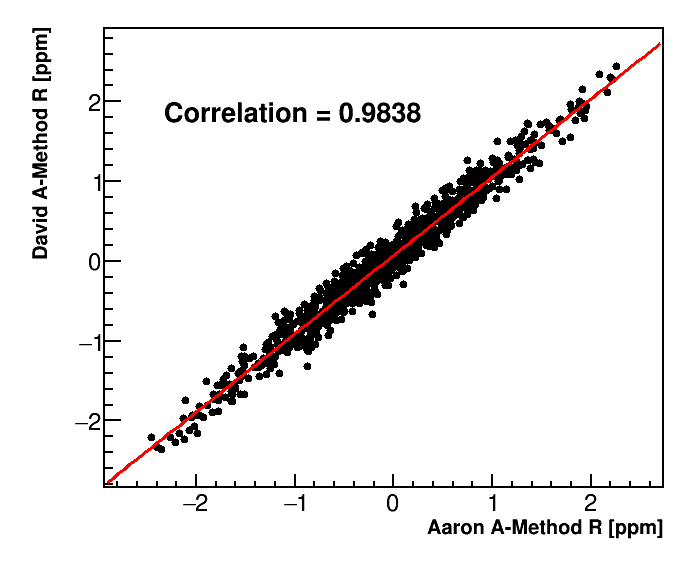
\includegraphics[width=\textwidth]{ScatterPlot}
\caption{from 9d dataset}
\label{fig:}
\end{figure}



\subsection{Correlation Results}



\begin{figure}[]
\centering
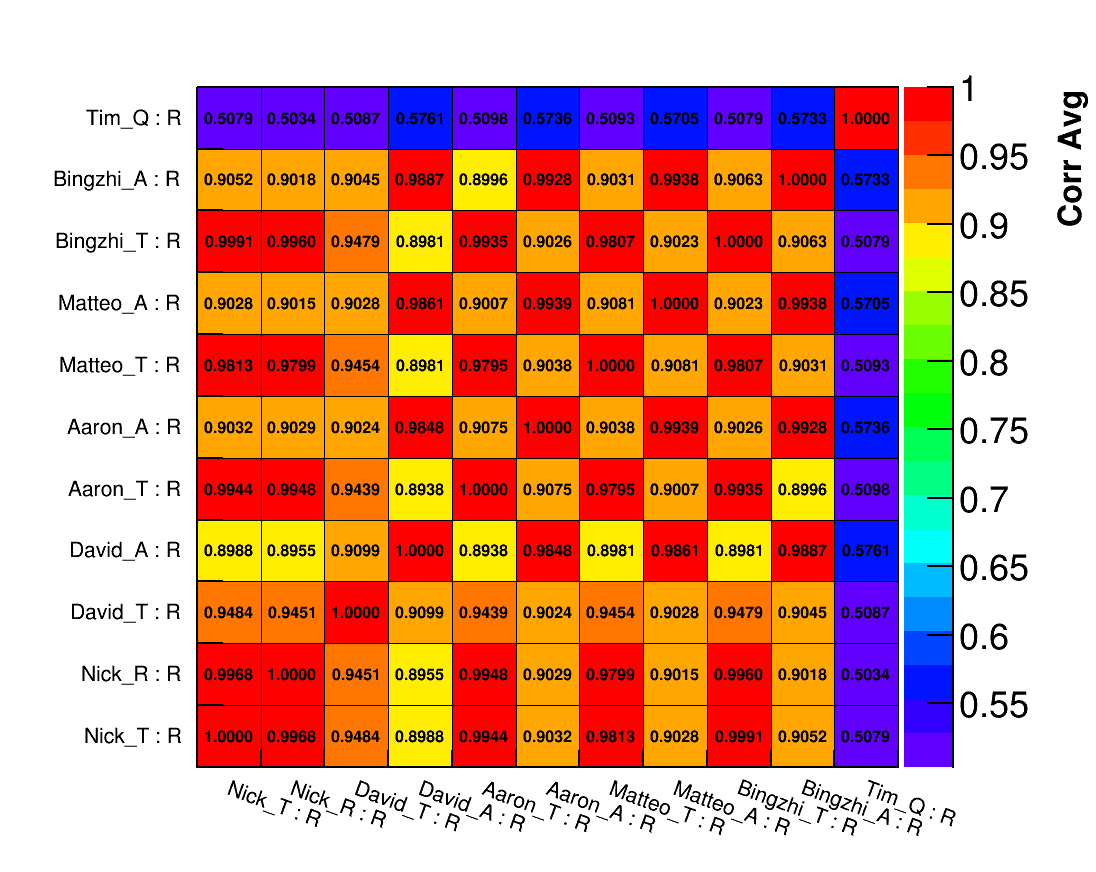
\includegraphics[width=\textwidth]{Avg_CorrelationMatrix_R_R}
\caption{EG}
\label{fig:}
\end{figure}

\begin{figure}[]
\centering
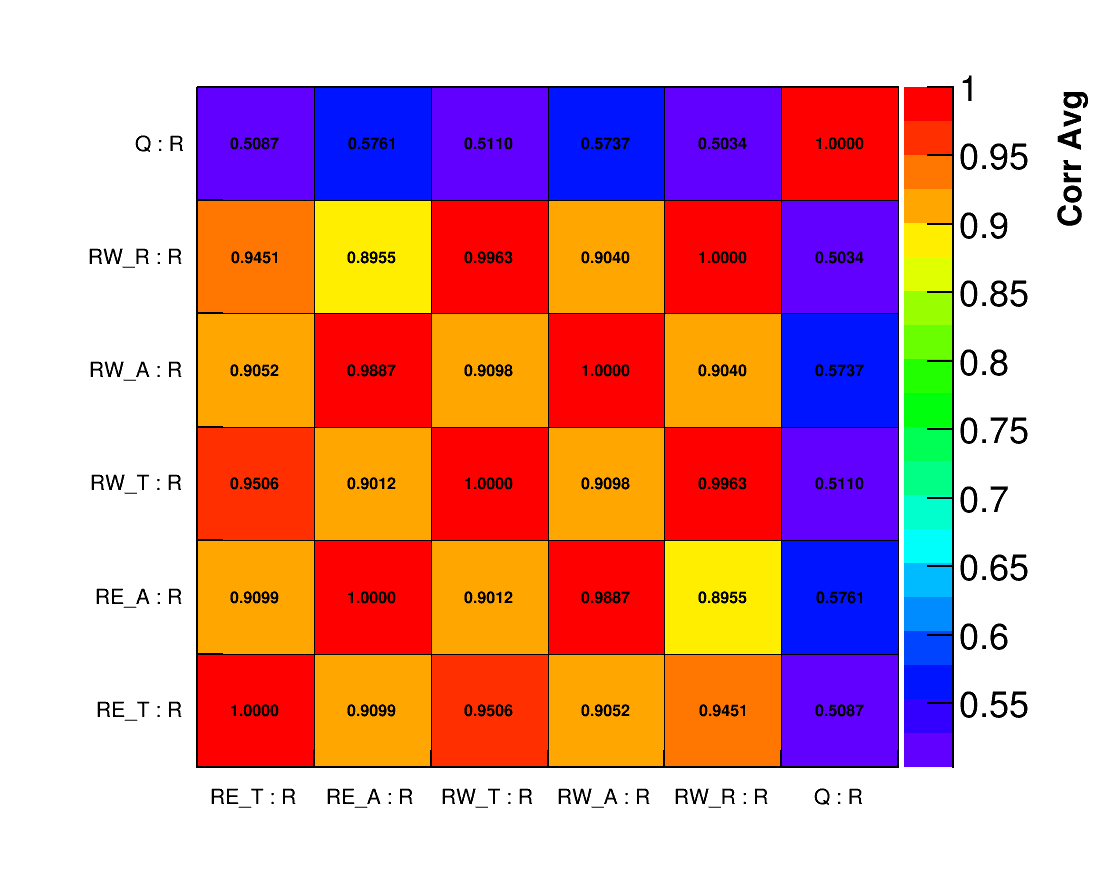
\includegraphics[width=\textwidth]{Avg_Recon_CorrelationMatrix_R_R}
\caption{EG}
\label{fig:}
\end{figure}


% 60h

\begin{landscape}
\begin{table}
\small
\centering
\renewcommand{\arraystretch}{1.5}
\begin{tabularx}{1\linewidth}{@{\extracolsep{\fill}}lXXXXXXXXXXX}
  \toprule
  	\multicolumn{12}{c}{{\normalsize 60h Correlation Coefficients -- Analyzer Level}} \\
  \midrule
  	       & BU T & BU R & CU T & CU A & UW T & UW A & EU T & EU A & SJTU T & SJTU A & UK Q \\
  \midrule
	BU T   & 1.0000 0.0000 & 0.9964 0.0001 & 0.9445 0.0015 & 0.8992 0.0016 & 0.9935 0.0001 & 0.8977 0.0004 & 0.9783 0.0001 & 0.9014 0.0002 & 0.9992 0.0001 & 0.9050 0.0004 & 0.5279 0.0208  \\
	BU R   & 0.9964 0.0001 & 1.0000 0.0000 & 0.9418 0.0018 & 0.8969 0.0020 & 0.9943 0.0001 & 0.8987 0.0008 & 0.9776 0.0004 & 0.9008 0.0007 & 0.9956 0.0001 & 0.9023 0.0010 & 0.5256 0.0203  \\
	CU T   & 0.9445 0.0015 & 0.9418 0.0018 & 1.0000 0.0000 & 0.9043 0.0010 & 0.9395 0.0013 & 0.8933 0.0024 & 0.9399 0.0019 & 0.8963 0.0021 & 0.9436 0.0015 & 0.8992 0.0021 & 0.5248 0.0176  \\
	CU A   & 0.8992 0.0016 & 0.8969 0.0020 & 0.9043 0.0010 & 1.0000 0.0000 & 0.8972 0.0003 & 0.9840 0.0001 & 0.8999 0.0021 & 0.9855 0.0003 & 0.8985 0.0022 & 0.9892 0.0004 & 0.5926 0.0227  \\
	UW T   & 0.9935 0.0001 & 0.9943 0.0001 & 0.9395 0.0013 & 0.8972 0.0003 & 1.0000 0.0000 & 0.9065 0.0010 & 0.9771 0.0001 & 0.9025 0.0012 & 0.9928 0.0001 & 0.9022 0.0010 & 0.5324 0.0229  \\
	UW A   & 0.8977 0.0004 & 0.8987 0.0008 & 0.8933 0.0024 & 0.9840 0.0001 & 0.9065 0.0010 & 1.0000 0.0000 & 0.9016 0.0005 & 0.9933 0.0002 & 0.8971 0.0006 & 0.9916 0.0002 & 0.5927 0.0300  \\
	EU T   & 0.9783 0.0001 & 0.9776 0.0004 & 0.9399 0.0019 & 0.8999 0.0021 & 0.9771 0.0001 & 0.9016 0.0005 & 1.0000 0.0000 & 0.9091 0.0003 & 0.9775 0.0001 & 0.9041 0.0004 & 0.5406 0.0262  \\
	EU A   & 0.9014 0.0002 & 0.9008 0.0007 & 0.8963 0.0021 & 0.9855 0.0003 & 0.9025 0.0012 & 0.9933 0.0002 & 0.9091 0.0003 & 1.0000 0.0000 & 0.9006 0.0004 & 0.9934 0.0001 & 0.5928 0.0306  \\
	SJTU T & 0.9992 0.0001 & 0.9956 0.0001 & 0.9436 0.0015 & 0.8985 0.0022 & 0.9928 0.0001 & 0.8971 0.0006 & 0.9775 0.0001 & 0.9006 0.0004 & 1.0000 0.0000 & 0.9058 0.0007 & 0.5271 0.0202  \\
	SJTU A & 0.9050 0.0004 & 0.9023 0.0010 & 0.8992 0.0021 & 0.9892 0.0004 & 0.9022 0.0010 & 0.9916 0.0002 & 0.9041 0.0004 & 0.9934 0.0001 & 0.9058 0.0007 & 1.0000 0.0000 & 0.5893 0.0274  \\
	UK Q   & 0.5279 0.0208 & 0.5256 0.0203 & 0.5248 0.0176 & 0.5926 0.0227 & 0.5324 0.0229 & 0.5927 0.0300 & 0.5406 0.0262 & 0.5928 0.0306 & 0.5271 0.0202 & 0.5893 0.0274 & 1.0000 0.0000  \\
  \bottomrule
\end{tabularx}
\caption[]{Correlation coefficients between \R values for the 60h dataset, at the analyzer level. In each table cell, the top number is the correlation coefficient and the bottom number is the error on the coefficient.}
\label{tab:Corrs_60h_analyzer}
\end{table}
\end{landscape}


\begin{table}
\setlength\tabcolsep{15pt}
\small
\centering
\renewcommand{\arraystretch}{1.4}
\begin{tabularx}{0.8\linewidth}{@{\extracolsep{\fill}}lXXXXXX}
  \toprule
  	\multicolumn{7}{c}{{\normalsize 60h Correlation Coefficients -- Recon. Level}} \\
  \midrule
  	       & RE T & RE A & RW T & RW A & RW R & \quad Q \\
  \midrule
	RE T   & 1.0000 0.0000 & 0.9043 0.0010 & 0.9467 0.0016 & 0.8984 0.0022 & 0.9418 0.0018 & 0.5248 0.0176  \\
	RE A   & 0.9043 0.0010 & 1.0000 0.0000 & 0.9033 0.0015 & 0.9886 0.0002 & 0.8969 0.0020 & 0.5926 0.0227  \\
	RW T   & 0.9467 0.0016 & 0.9033 0.0015 & 1.0000 0.0000 & 0.9097 0.0002 & 0.9961 0.0001 & 0.5348 0.0227  \\
	RW A   & 0.8984 0.0022 & 0.9886 0.0002 & 0.9097 0.0002 & 1.0000 0.0000 & 0.9028 0.0008 & 0.5930 0.0294  \\
	RW R   & 0.9418 0.0018 & 0.8969 0.0020 & 0.9961 0.0001 & 0.9028 0.0008 & 1.0000 0.0000 & 0.5256 0.0203  \\
	Q      & 0.5248 0.0176 & 0.5926 0.0227 & 0.5348 0.0227 & 0.5930 0.0294 & 0.5256 0.0203 & 1.0000 0.0000  \\
  \bottomrule
\end{tabularx}
\caption[]{Correlation coefficients between \R values for the 60h dataset, at the reconstruction level after the \RW T-Method and A-Method \R values were averaged among the different analyzers. In each table cell, the top number is the correlation coefficient and the bottom number is the error on the coefficient.}
\label{tab:Corrs_60h_recon}
\end{table}


% HK

\begin{landscape}
\begin{table}
\small
\centering
\renewcommand{\arraystretch}{1.5}
\begin{tabularx}{1\linewidth}{@{\extracolsep{\fill}}lXXXXXXXXXXX}
  \toprule
  	\multicolumn{12}{c}{{\normalsize HK Correlation Coefficients -- Analyzer Level}} \\
  \midrule
  	       & BU T & BU R & CU T & CU A & UW T & UW A & EU T & EU A & SJTU T & SJTU A & UK Q \\
  \midrule
	BU T   & 1.0000 0.0000 & 0.9967 0.0001 & 0.9469 0.0023 & 0.8924 0.0042 & 0.9939 0.0003 & 0.8938 0.0015 & 0.9799 0.0011 & 0.8946 0.0031 & 0.9992 0.0001 & 0.8978 0.0033 & 0.4982 0.0057  \\
	BU R   & 0.9967 0.0001 & 1.0000 0.0000 & 0.9439 0.0024 & 0.8907 0.0047 & 0.9943 0.0003 & 0.8955 0.0018 & 0.9785 0.0010 & 0.8948 0.0035 & 0.9958 0.0001 & 0.8959 0.0036 & 0.4959 0.0070  \\
	CU T   & 0.9469 0.0023 & 0.9439 0.0024 & 1.0000 0.0000 & 0.8968 0.0027 & 0.9408 0.0028 & 0.8858 0.0002 & 0.9409 0.0012 & 0.8865 0.0010 & 0.9458 0.0025 & 0.8900 0.0015 & 0.4913 0.0114  \\
	CU A   & 0.8924 0.0042 & 0.8907 0.0047 & 0.8968 0.0027 & 1.0000 0.0000 & 0.8872 0.0058 & 0.9839 0.0010 & 0.8900 0.0026 & 0.9846 0.0004 & 0.8913 0.0045 & 0.9892 0.0003 & 0.5635 0.0137  \\
	UW T   & 0.9939 0.0003 & 0.9943 0.0003 & 0.9408 0.0028 & 0.8872 0.0058 & 1.0000 0.0000 & 0.8993 0.0019 & 0.9776 0.0020 & 0.8928 0.0042 & 0.9930 0.0002 & 0.8920 0.0046 & 0.5015 0.0021  \\
	UW A   & 0.8938 0.0015 & 0.8955 0.0018 & 0.8858 0.0002 & 0.9839 0.0010 & 0.8993 0.0019 & 1.0000 0.0000 & 0.8943 0.0008 & 0.9935 0.0005 & 0.8928 0.0018 & 0.9918 0.0005 & 0.5642 0.0115  \\
	EU T   & 0.9799 0.0011 & 0.9785 0.0010 & 0.9409 0.0012 & 0.8900 0.0026 & 0.9776 0.0020 & 0.8943 0.0008 & 1.0000 0.0000 & 0.8998 0.0014 & 0.9791 0.0012 & 0.8949 0.0018 & 0.5066 0.0020  \\
	EU A   & 0.8946 0.0031 & 0.8948 0.0035 & 0.8865 0.0010 & 0.9846 0.0004 & 0.8928 0.0042 & 0.9935 0.0005 & 0.8998 0.0014 & 1.0000 0.0000 & 0.8936 0.0035 & 0.9935 0.0001 & 0.5637 0.0121  \\
	SJTU T & 0.9992 0.0001 & 0.9958 0.0001 & 0.9458 0.0025 & 0.8913 0.0045 & 0.9930 0.0002 & 0.8928 0.0018 & 0.9791 0.0012 & 0.8936 0.0035 & 1.0000 0.0000 & 0.8984 0.0037 & 0.4987 0.0059  \\
	SJTU A & 0.8978 0.0033 & 0.8959 0.0036 & 0.8900 0.0015 & 0.9892 0.0003 & 0.8920 0.0046 & 0.9918 0.0005 & 0.8949 0.0018 & 0.9935 0.0001 & 0.8984 0.0037 & 1.0000 0.0000 & 0.5612 0.0141  \\
	UK Q   & 0.4982 0.0057 & 0.4959 0.0070 & 0.4913 0.0114 & 0.5635 0.0137 & 0.5015 0.0021 & 0.5642 0.0115 & 0.5066 0.0020 & 0.5637 0.0121 & 0.4987 0.0059 & 0.5612 0.0141 & 1.0000 0.0000  \\
  \bottomrule
\end{tabularx}
\caption[]{Correlation coefficients between \R values for the HK dataset, at the analyzer level. In each table cell, the top number is the correlation coefficient and the bottom number is the error on the coefficient.}
\label{tab:Corrs_HK_analyzer}
\end{table}
\end{landscape}


\begin{table}
\setlength\tabcolsep{15pt}
\small
\centering
\renewcommand{\arraystretch}{1.4}
\begin{tabularx}{0.8\linewidth}{@{\extracolsep{\fill}}lXXXXXX}
  \toprule
  	\multicolumn{7}{c}{{\normalsize HK Correlation Coefficients -- Recon. Level}} \\
  \midrule
  	       & RE T & RE A & RW T & RW A & RW R & \quad Q \\
  \midrule
	RE T   & 1.0000 0.0000 & 0.8968 0.0027 & 0.9482 0.0019 & 0.8896 0.0007 & 0.9439 0.0024 & 0.4913 0.0114  \\
	RE A   & 0.8968 0.0027 & 1.0000 0.0000 & 0.8946 0.0040 & 0.9883 0.0005 & 0.8907 0.0047 & 0.5635 0.0137  \\
	RW T   & 0.9482 0.0019 & 0.8946 0.0040 & 1.0000 0.0000 & 0.9018 0.0023 & 0.9962 0.0001 & 0.5037 0.0032  \\
	RW A   & 0.8896 0.0007 & 0.9883 0.0005 & 0.9018 0.0023 & 1.0000 0.0000 & 0.8975 0.0029 & 0.5643 0.0127  \\
	RW R   & 0.9439 0.0024 & 0.8907 0.0047 & 0.9962 0.0001 & 0.8975 0.0029 & 1.0000 0.0000 & 0.4959 0.0070  \\
	Q      & 0.4913 0.0114 & 0.5635 0.0137 & 0.5037 0.0032 & 0.5643 0.0127 & 0.4959 0.0070 & 1.0000 0.0000  \\
  \bottomrule
\end{tabularx}
\caption[]{Correlation coefficients between \R values for the HK dataset, at the reconstruction level after the \RW T-Method and A-Method \R values were averaged among the different analyzers. In each table cell, the top number is the correlation coefficient and the bottom number is the error on the coefficient.}
\label{tab:Corrs_HK_recon}
\end{table}


% 9d


\begin{landscape}
\begin{table}
\small
\centering
\renewcommand{\arraystretch}{1.5}
\begin{tabularx}{1\linewidth}{@{\extracolsep{\fill}}lXXXXXXXXXXX}
  \toprule
  	\multicolumn{12}{c}{{\normalsize 9d Correlation Coefficients -- Analyzer Level}} \\
  \midrule
  	       & BU T & BU R & CU T & CU A & UW T & UW A & EU T & EU A & SJTU T & SJTU A & UK Q \\
  \midrule
	BU T   & 1.0000 0.0000 & 0.9965 0.0003 & 0.9445 0.0015 & 0.8912 0.0087 & 0.9939 0.0005 & 0.8935 0.0058 & 0.9787 0.0018 & 0.8952 0.0082 & 0.9993 0.0001 & 0.8983 0.0071 & 0.4936 0.0105  \\
	BU R   & 0.9965 0.0003 & 1.0000 0.0000 & 0.9414 0.0018 & 0.8885 0.0097 & 0.9944 0.0004 & 0.8944 0.0061 & 0.9782 0.0011 & 0.8945 0.0084 & 0.9958 0.0003 & 0.8957 0.0077 & 0.4888 0.0109  \\
	CU T   & 0.9445 0.0015 & 0.9414 0.0018 & 1.0000 0.0000 & 0.9002 0.0022 & 0.9392 0.0025 & 0.8905 0.0007 & 0.9419 0.0011 & 0.8906 0.0018 & 0.9438 0.0019 & 0.8944 0.0017 & 0.5000 0.0071  \\
	CU A   & 0.8912 0.0087 & 0.8885 0.0097 & 0.9002 0.0022 & 1.0000 0.0000 & 0.8861 0.0102 & 0.9833 0.0005 & 0.8904 0.0059 & 0.9840 0.0005 & 0.8903 0.0090 & 0.9886 0.0006 & 0.5710 0.0007  \\
	UW T   & 0.9939 0.0005 & 0.9944 0.0004 & 0.9392 0.0025 & 0.8861 0.0102 & 1.0000 0.0000 & 0.8990 0.0068 & 0.9770 0.0011 & 0.8931 0.0098 & 0.9931 0.0005 & 0.8929 0.0089 & 0.4999 0.0128  \\
	UW A   & 0.8935 0.0058 & 0.8944 0.0061 & 0.8905 0.0007 & 0.9833 0.0005 & 0.8990 0.0068 & 1.0000 0.0000 & 0.8966 0.0032 & 0.9932 0.0002 & 0.8926 0.0060 & 0.9923 0.0002 & 0.5750 0.0031  \\
	EU T   & 0.9787 0.0018 & 0.9782 0.0011 & 0.9419 0.0011 & 0.8904 0.0059 & 0.9770 0.0011 & 0.8966 0.0032 & 1.0000 0.0000 & 0.9021 0.0056 & 0.9778 0.0019 & 0.8974 0.0053 & 0.4992 0.0042  \\
	EU A   & 0.8952 0.0082 & 0.8945 0.0084 & 0.8906 0.0018 & 0.9840 0.0005 & 0.8931 0.0098 & 0.9932 0.0002 & 0.9021 0.0056 & 1.0000 0.0000 & 0.8944 0.0083 & 0.9940 0.0002 & 0.5698 0.0015  \\
	SJTU T & 0.9993 0.0001 & 0.9958 0.0003 & 0.9438 0.0019 & 0.8903 0.0090 & 0.9931 0.0005 & 0.8926 0.0060 & 0.9778 0.0019 & 0.8944 0.0083 & 1.0000 0.0000 & 0.8988 0.0074 & 0.4913 0.0108  \\
	SJTU A & 0.8983 0.0071 & 0.8957 0.0077 & 0.8944 0.0017 & 0.9886 0.0006 & 0.8929 0.0089 & 0.9923 0.0002 & 0.8974 0.0053 & 0.9940 0.0002 & 0.8988 0.0074 & 1.0000 0.0000 & 0.5651 0.0011  \\
	UK Q   & 0.4936 0.0105 & 0.4888 0.0109 & 0.5000 0.0071 & 0.5710 0.0007 & 0.4999 0.0128 & 0.5750 0.0031 & 0.4992 0.0042 & 0.5698 0.0015 & 0.4913 0.0108 & 0.5651 0.0011 & 1.0000 0.0000  \\
  \bottomrule
\end{tabularx}
\caption[]{Correlation coefficients between \R values for the 9d dataset, at the analyzer level. In each table cell, the top number is the correlation coefficient and the bottom number is the error on the coefficient.}
\label{tab:Corrs_9d_analyzer}
\end{table}
\end{landscape}


\begin{table}
\setlength\tabcolsep{15pt}
\small
\centering
\renewcommand{\arraystretch}{1.4}
\begin{tabularx}{0.8\linewidth}{@{\extracolsep{\fill}}lXXXXXX}
  \toprule
  	\multicolumn{7}{c}{{\normalsize 9d Correlation Coefficients -- Recon. Level}} \\
  \midrule
  	       & RE T & RE A & RW T & RW A & RW R & \quad Q \\
  \midrule
	RE T   & 1.0000 0.0000 & 0.9002 0.0022 & 0.9471 0.0014 & 0.8939 0.0014 & 0.9414 0.0018 & 0.5000 0.0071  \\
	RE A   & 0.9002 0.0022 & 1.0000 0.0000 & 0.8940 0.0082 & 0.9876 0.0005 & 0.8885 0.0097 & 0.5710 0.0007  \\
	RW T   & 0.9471 0.0014 & 0.8940 0.0082 & 1.0000 0.0000 & 0.9027 0.0066 & 0.9963 0.0002 & 0.4985 0.0074  \\
	RW A   & 0.8939 0.0014 & 0.9876 0.0005 & 0.9027 0.0066 & 1.0000 0.0000 & 0.8969 0.0074 & 0.5713 0.0011  \\
	RW R   & 0.9414 0.0018 & 0.8885 0.0097 & 0.9963 0.0002 & 0.8969 0.0074 & 1.0000 0.0000 & 0.4888 0.0109  \\
	Q      & 0.5000 0.0071 & 0.5710 0.0007 & 0.4985 0.0074 & 0.5713 0.0011 & 0.4888 0.0109 & 1.0000 0.0000  \\
  \bottomrule
\end{tabularx}
\caption[]{Correlation coefficients between \R values for the 9d dataset, at the reconstruction level after the \RW T-Method and A-Method \R values were averaged among the different analyzers. In each table cell, the top number is the correlation coefficient and the bottom number is the error on the coefficient.}
\label{tab:Corrs_9d_recon}
\end{table}


% EG


\begin{landscape}
\begin{table}
\small
\centering
\renewcommand{\arraystretch}{1.5}
\begin{tabularx}{1\linewidth}{@{\extracolsep{\fill}}lXXXXXXXXXXX}
  \toprule
  	\multicolumn{12}{c}{{\normalsize EG Correlation Coefficients -- Analyzer Level}} \\
  \midrule
  	       & BU T & BU R & CU T & CU A & UW T & UW A & EU T & EU A & SJTU T & SJTU A & UK Q \\
  \midrule
	BU T   & 1.0000 0.0000 & 0.9968 0.0001 & 0.9484 0.0020 & 0.8988 0.0091 & 0.9944 0.0004 & 0.9032 0.0073 & 0.9813 0.0004 & 0.9028 0.0086 & 0.9991 0.0001 & 0.9052 0.0088 & 0.5079 0.0104  \\
	BU R   & 0.9968 0.0001 & 1.0000 0.0000 & 0.9451 0.0025 & 0.8955 0.0102 & 0.9948 0.0006 & 0.9029 0.0087 & 0.9799 0.0007 & 0.9015 0.0096 & 0.9960 0.0001 & 0.9018 0.0099 & 0.5034 0.0099  \\
	CU T   & 0.9484 0.0020 & 0.9451 0.0025 & 1.0000 0.0000 & 0.9099 0.0025 & 0.9439 0.0019 & 0.9024 0.0008 & 0.9454 0.0032 & 0.9028 0.0010 & 0.9479 0.0016 & 0.9045 0.0005 & 0.5087 0.0090  \\
	CU A   & 0.8988 0.0091 & 0.8955 0.0102 & 0.9099 0.0025 & 1.0000 0.0000 & 0.8938 0.0099 & 0.9848 0.0005 & 0.8981 0.0105 & 0.9861 0.0002 & 0.8981 0.0092 & 0.9887 0.0006 & 0.5761 0.0012  \\
	UW T   & 0.9944 0.0004 & 0.9948 0.0006 & 0.9439 0.0019 & 0.8938 0.0099 & 1.0000 0.0000 & 0.9075 0.0079 & 0.9795 0.0010 & 0.9007 0.0095 & 0.9935 0.0005 & 0.8996 0.0100 & 0.5098 0.0102  \\
	UW A   & 0.9032 0.0073 & 0.9029 0.0087 & 0.9024 0.0008 & 0.9848 0.0005 & 0.9075 0.0079 & 1.0000 0.0000 & 0.9038 0.0088 & 0.9939 0.0004 & 0.9026 0.0072 & 0.9928 0.0004 & 0.5736 0.0038  \\
	EU T   & 0.9813 0.0004 & 0.9799 0.0007 & 0.9454 0.0032 & 0.8981 0.0105 & 0.9795 0.0010 & 0.9038 0.0088 & 1.0000 0.0000 & 0.9081 0.0096 & 0.9807 0.0004 & 0.9031 0.0096 & 0.5093 0.0083  \\
	EU A   & 0.9028 0.0086 & 0.9015 0.0096 & 0.9028 0.0010 & 0.9861 0.0002 & 0.9007 0.0095 & 0.9939 0.0004 & 0.9081 0.0096 & 1.0000 0.0000 & 0.9023 0.0086 & 0.9938 0.0002 & 0.5705 0.0034  \\
	SJTU T & 0.9991 0.0001 & 0.9960 0.0001 & 0.9479 0.0016 & 0.8981 0.0092 & 0.9935 0.0005 & 0.9026 0.0072 & 0.9807 0.0004 & 0.9023 0.0086 & 1.0000 0.0000 & 0.9063 0.0086 & 0.5079 0.0110  \\
	SJTU A & 0.9052 0.0088 & 0.9018 0.0099 & 0.9045 0.0005 & 0.9887 0.0006 & 0.8996 0.0100 & 0.9928 0.0004 & 0.9031 0.0096 & 0.9938 0.0002 & 0.9063 0.0086 & 1.0000 0.0000 & 0.5733 0.0013  \\
	UK Q   & 0.5079 0.0104 & 0.5034 0.0099 & 0.5087 0.0090 & 0.5761 0.0012 & 0.5098 0.0102 & 0.5736 0.0038 & 0.5093 0.0083 & 0.5705 0.0034 & 0.5079 0.0110 & 0.5733 0.0013 & 1.0000 0.0000  \\
  \bottomrule
\end{tabularx}
\caption[]{Correlation coefficients between \R values for the EG dataset, at the analyzer level. In each table cell, the top number is the correlation coefficient and the bottom number is the error on the coefficient.}
\label{tab:Corrs_EG_analyzer}
\end{table}
\end{landscape}


\begin{table}
\setlength\tabcolsep{15pt}
\small
\centering
\renewcommand{\arraystretch}{1.4}
\begin{tabularx}{0.8\linewidth}{@{\extracolsep{\fill}}lXXXXXX}
  \toprule
  	\multicolumn{7}{c}{{\normalsize EG Correlation Coefficients -- Recon. Level}} \\
  \midrule
  	       & RE T & RE A & RW T & RW A & RW R & \quad Q \\
  \midrule
	RE T   & 1.0000 0.0000 & 0.9099 0.0025 & 0.9506 0.0020 & 0.9052 0.0002 & 0.9451 0.0025 & 0.5087 0.0090  \\
	RE A   & 0.9099 0.0025 & 1.0000 0.0000 & 0.9012 0.0096 & 0.9887 0.0003 & 0.8955 0.0102 & 0.5761 0.0012  \\
	RW T   & 0.9506 0.0020 & 0.9012 0.0096 & 1.0000 0.0000 & 0.9098 0.0085 & 0.9963 0.0002 & 0.5110 0.0101  \\
	RW A   & 0.9052 0.0002 & 0.9887 0.0003 & 0.9098 0.0085 & 1.0000 0.0000 & 0.9040 0.0093 & 0.5737 0.0029  \\
	RW R   & 0.9451 0.0025 & 0.8955 0.0102 & 0.9963 0.0002 & 0.9040 0.0093 & 1.0000 0.0000 & 0.5034 0.0099  \\
	Q      & 0.5087 0.0090 & 0.5761 0.0012 & 0.5110 0.0101 & 0.5737 0.0029 & 0.5034 0.0099 & 1.0000 0.0000  \\
  \bottomrule
\end{tabularx}
\caption[]{Correlation coefficients between \R values for the EG dataset, at the reconstruction level after the \RW T-Method and A-Method \R values were averaged among the different analyzers. In each table cell, the top number is the correlation coefficient and the bottom number is the error on the coefficient.}
\label{tab:Corrs_EG_recon}
\end{table}


